\section{Front-end}
\label{sec:front-end}

\subsection{Initial Ideas}
We quickly realised that our ideas could easily expand the project, with numerous functionality and features, that would bring the project to a far too complex level.
We mapped all our ideas and prioritized them, and made a selection of ideas, which we planned on implementing.

\begin{figure}[ht]
\centering
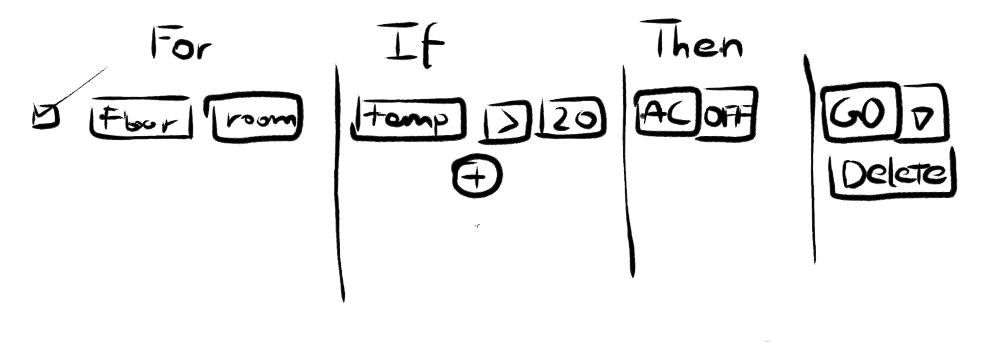
\includegraphics[width=\columnwidth]{initial_idea_frontend.png}
\caption{Initial drawing.}
\label{fig:initialidea}
\end{figure}

The selected ideas that we wanted to realise (sorted by importance) included:
\begin{itemize}
\item Users should be able to add, delete and modify policies.
\item Users should be able to use complex operators in policies, e.g. higher than, lower than, equal to etc.
\item Users should be able to save policies and easily toggle an ON or OFF state.
\item Users should be able to combine multiple sensors in a single policy.
%%%% Aslak: Remember to describe how these wildcards are implemented. In the proper section.
\item Users should be able to use wildcards in a policy, e.g. effecting for instance an entire floor without the need to specify the rooms that belong to the chosen floor.
\item Users should be able to create nested rules in policies.
\end{itemize}

\begin{figure}[ht]
\centering
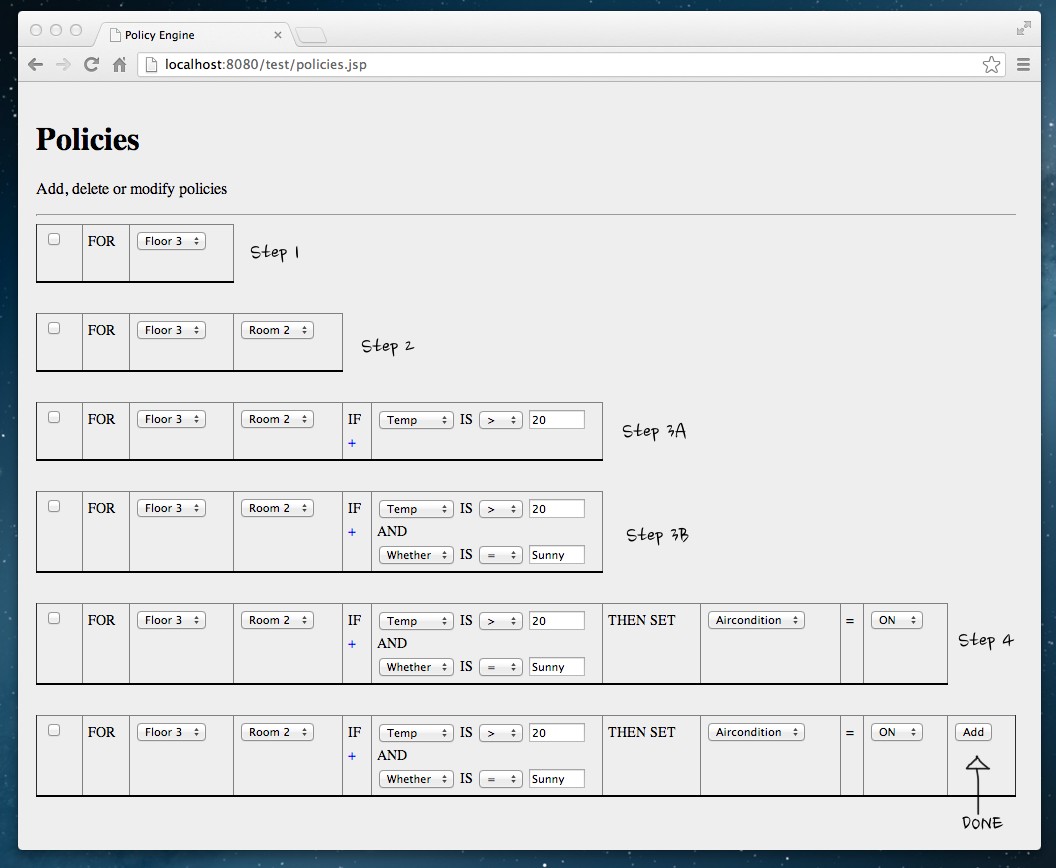
\includegraphics[width=\columnwidth]{building_policy_steps.png}
\caption{Initial drawing - step wise build up.}
\label{fig:initialidea:policysteps}
\end{figure}

All these points where realised in the backend of our implementation, however because of time limits we regret that the possibility to create nested statements did not make it to the user interface. Still we have an interface fully ready to support nested statements, but this is something we have added to future work instead. We have started work on a recursive function to be able to cleverly support endlessly (in theory, computing resources are not endless) deep nested statements. These nested statements would be listed under THEN and would contain a new set of IF, THEN, ELSE subsections. These sections would be easy readable because of indentation and encapsulation.

\subsection{User Interface}
The main goal for the user interface has been to keep it simple and user-friendly without loosing advanced functionality. Initially we started making rough drawings to better understand what we were dealing with and how to best possibly present it. Doing so we tried to sketch the process of handling a policy from the creation to the enabling of it. We came up with various approaches one of the more interesting ones being the step wise (see figures \ref{fig:initialidea}, \ref{fig:initialidea:policysteps}). However this approach proved to not be as flexible and able to handle very detailed and complex polices. Our aim has been to make a great overview for the user. Therefor we chose another concept that are splitting each statement up into an open / closeable area to better encapsulate the logic. We found that you very often read one statement at a time, therefor you can have the statements open you are interested in, and won't be confused by statements not applicable to an area of interest. Within each statement we also decided to split up IF, THEN and ELSE into subsections because you in theory can add as many entries to each subsection as needed. Nonetheless the introduction of "`wildcard"' values for instance allows to manipulate an entire floors heaters, taking up much less space and work for the user to define then having to set up entries for each heater on a floor. See an example from the final view of a policy build at figure \ref{fig:statement}.

\subsubsection{Intuitive Design}
What you want to achieve when designing an interface is to make it as intuitive as possible. This can be archieved by looking at the user's "knowledge space" \cite{intuitivedesign}.

\begin{figure}[ht]
\centering
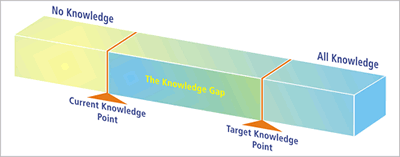
\includegraphics[width=\columnwidth]{knowledge-brick-3.png}
\caption{The space between the Current Knowledge and Target Knowledge points is called The Knowledge Gap.}
\label{fig:intuitivedesign}
\end{figure}

The distance from the left (As seen on figure \ref{fig:intuitivedesign}) indicates how much a given user is familiar with an interface, this is called the "current knowledge point". The next point of interest is called "target knowledge point". This section details how much knowledge the user needs to know to achieve their goals.
Each time a user attempts to perform a specific task, their "current knowledge point" and "target knowledge point" are very important for us to identify.
Each user's "current knowledge point" and "target knowledge point" will be different when they gain more experience. However, it turns out that, by making usability tests we can often identify groups of users who have almost the same "current knowledge point". This is also why we have performed think-aloud tests, which we will get back to later in this report.

"The Knowledge Gap", which is the distance between the "current knowledge point" and the "target knowledge point", is also called "The Gap".
"The Gap" is what you have full focus on designing for. There is no need to design to the left of the "current knowledge point" and you do not need to design to the right of the "target knowledge point" since the user does not need the knowledge to perform the task. One should therefore focus only on designing the interface for the space in between the two points.

Users can accomplish their goals when the "current knowledge point" is equal to the "target knowledge point". There are two ways to achieve this. You can train the user, thereby increasing their current knowledge, until they know everything they need to do the job. The other way is to design an interface that can reduce the "current knowledge point" by making the interface more accessible until the "target knowledge point" requires only the information the user already has.


\subsubsection{Speed}
You need speed to save time! Therefore if your application takes 5 seconds every time someone clicks a button to load a page then that is bad! When a user sets up a policy, then they want to have it done in a fast and easy way. If the majority of the time is spent loading the page or saving updates all the time the users will simply not use the application. Therefor we have made a interface using Javascript / Jquery that lets the user setup and model any changes almost instantly before saving it to the database. This way they can experiment and set statements up without overwriting the policy until they are sure they want to save what they have done.

\subsubsection{Color Coding}
It's important to use color in your interface. Colors send signals to the user sub-consciously, so therefore you can make use of this with things like buttons and colored areas. We have used this idea to color the different boxes under a statement, to improve the readability and make it more intuitive. We used a red color for the IF boxes and a green color for the THEN and ELSE boxes. The reason for this is that the IF is a "`get"' type and the other two is a "`set"' type.

\subsubsection{Responsive Design}
Responsive web design is a web design approach aimed at crafting sites to provide an optimal viewing experience—easy reading and navigation with a minimum of resizing, panning, and scrolling—across a wide range of devices (from desktop computer monitors to mobile phones). While we haven't directly optimized for mobile we have had the responsive design idea in mind when setting up the design. What we have assured is that the user interface is adjusted to the screen size of the user. Meaning if you for instance use a full HD resolution (1920x1080) the interface will utilize this space (see examples on figures \ref{fig:policylist}, \ref{fig:policy}, \ref{fig:statement}).

\begin{figure}[ht]
\centering
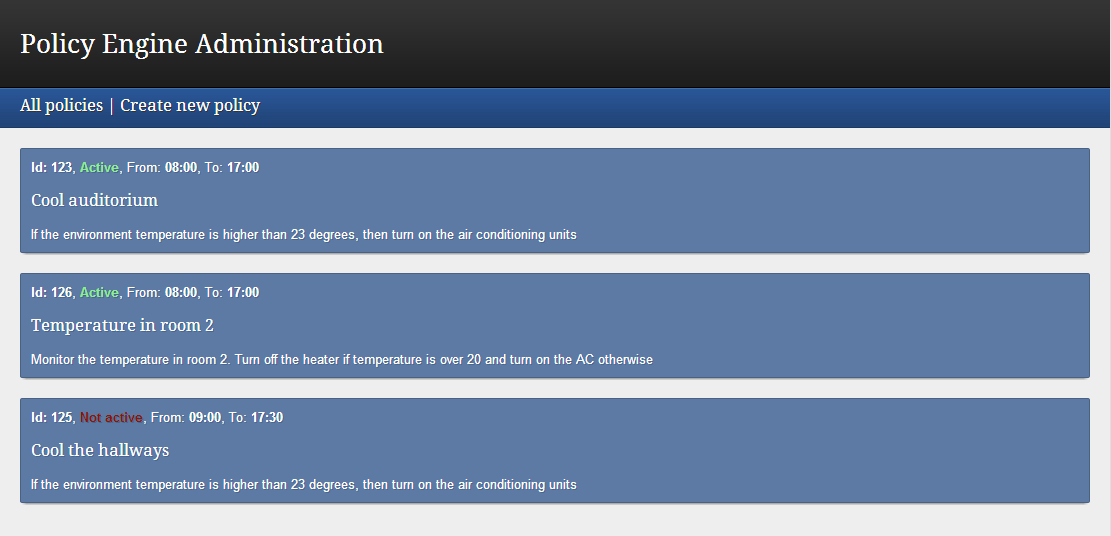
\includegraphics[width=\columnwidth]{policylist.png}
\caption{Illustrating the policy list-view.}
\label{fig:policylist}
\end{figure}

\subsection{Policy Editor}

\subsubsection{Managing Policies}
In order to make it simple and fast to manage a policy we have split the interface for a policy up into sections and sub sections. We have two sections: Policy Information and Policy Statements. In Policy Information, all the content: name, description and time interval are defined. Also if the policy should be active, and run on the Policy Engine, can be defined in this section. The Policy Statements section is where all the conditions and actions are defined. We have added a sub section for each statement to improve the readability and overview of what is executed and what is paired together (see figure \ref{fig:policy}).  

\begin{figure}[ht]
\centering
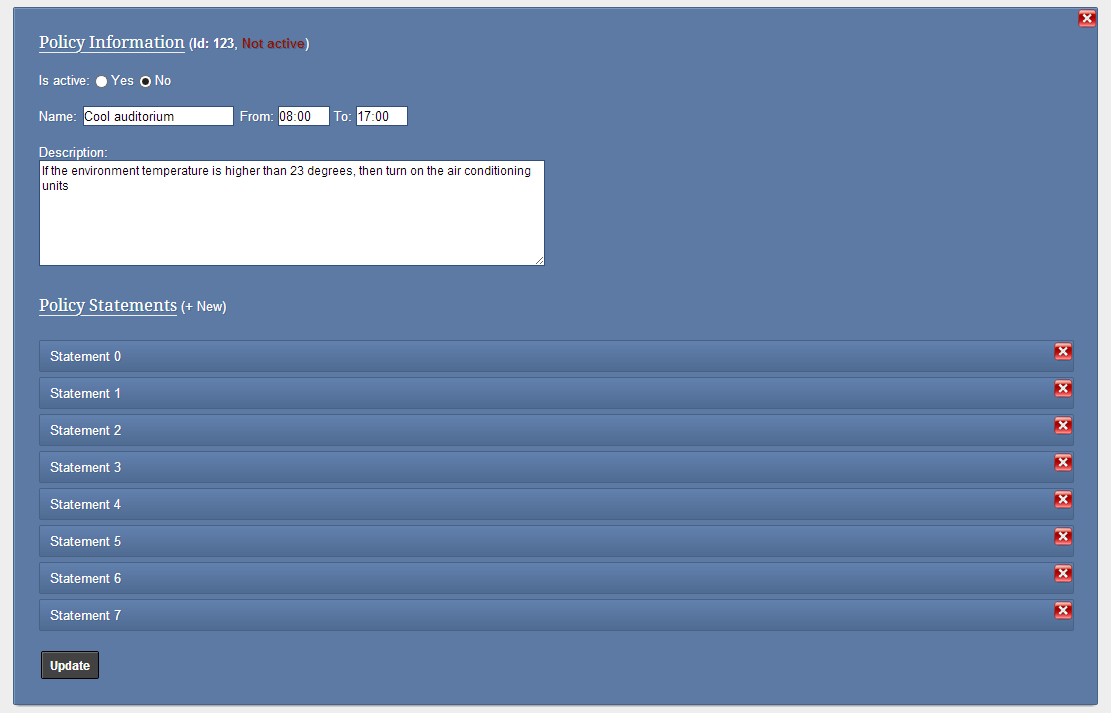
\includegraphics[width=\columnwidth]{policy.png}
\caption{Editing a policy.}
\label{fig:policy}
\end{figure}

Within a statement there are three sub sections: IF, THEN, ELSE (see figure \ref{fig:statement}). For each headline in this setup there is a "`+ New"' button that can be clicked. This will add a new entry to this particular area. While this is done we alter the policy object in the background so once the user are satisfied with the setup of statements, it can be saved with a click on the update / save button.

To help the user find the correct sensor / wildcard option, we have implemented an autocomplete functionality. This lets the user start typing a value and then the autocomplete will come up with all the matching elements available.

To make it take less space and work to define a statement that should apply to an entire floor or room, we have introduced wildcard options. A use case can for instance be: A user wants to work with the blinds on the entire first floor: floor1-blinds is then the option to pick.

\begin{figure}[ht]
\centering
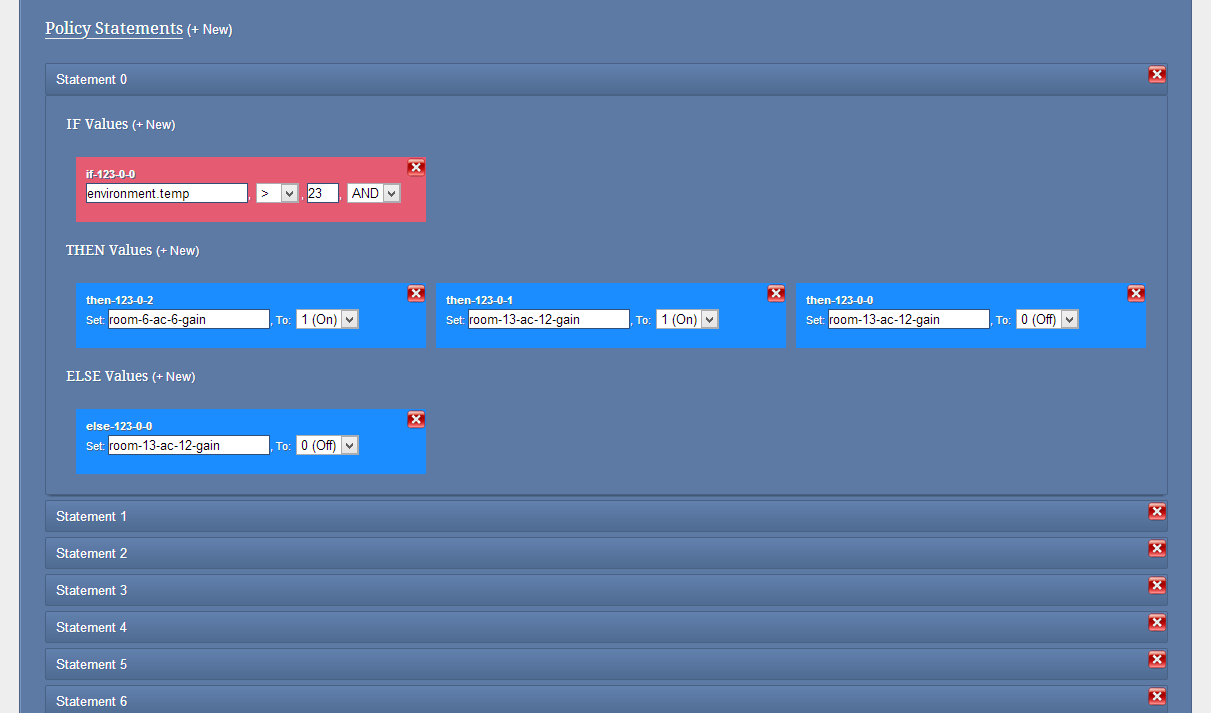
\includegraphics[width=\columnwidth]{statement.png}
\caption{Configuring statements.}
\label{fig:statement}
\end{figure}

\subsection{Use Case View}
The solution's final use case diagram is shown in Figure \ref{fig:usecasediagram}.

\begin{figure}[ht]
\centering
%\includegraphics[width=\columnwidth]{usecasediagram.png}
\caption{Use Case Diagram (that is missing!)}
\label{fig:usecasediagram}
\end{figure}

% ATTENTION: Short description of usecase

\subsection{Usability}
Seeing policies as rules for rooms in a building, with multiple sensors in each and every room, that can affect multiple actuators - not only in one room, but all of the rooms in a building: It leaves the user with a lot of selections. 
This will, if not represented properly, complicate the process of adding new policies.

Following the principles of Steve Krug's "Don't Make Me Think: Common Sense Approach to the Web"\cite{Krug:2005:DMM:1051204}, the functionality of a website should always let users accomplish their intended tasks as easy and directly as possible.
Throughout the development of the front end site we have thrived to do so. And we have had two usability tests (more on this in the \nameref{chapter:evaluation} part) to uncover potential problems.

\subsubsection{Browser Compatibility}
We have optimized for modern web browsers. The specific browsers we have tested our solution in are: Internet Explorer 9 and 10, Firefox, Chrome, Safari. 

\subsubsection{Layers of Abstraction}
With the policy engine there are different layers of abstraction: Visual UI, Textual UI, Engine.

We have focused on the Visual UI enabling a graphical representation of the CRUD process. The other approach is having policies handled in a textual manner, and thereby forcing users to a write the statements in a policy, using a domain specific language. For a developer textual editing and console commands might be preferred, and may somewhat be quicker, while they know the inputs by heart. But the intended users of our policy engine, are most likely not developers or fans of typing in commands.

In a future version of the policy engine, both methods could be implemented to function in parallel, giving a user both choices, and also the capability of copy and paste policies quickly.